\documentclass[11pt]{article}

\usepackage[a4paper,margin=2.3cm]{geometry}
\usepackage{graphicx}
\usepackage{float}
\usepackage{booktabs}
\usepackage{multirow}
\usepackage{amsmath}
\usepackage{amssymb}
\usepackage{caption}
\usepackage{subcaption}
\usepackage{xcolor}
\usepackage{array}
\usepackage{longtable}
\usepackage{tikz}
\usepackage[hidelinks]{hyperref}

\usetikzlibrary{patterns,arrows.meta}

\graphicspath{{figures/}{../output/column/}}

\captionsetup{font=small,labelfont=bf}
\setlength{\parindent}{0pt}
\setlength{\parskip}{4pt}
\setlength{\emergencystretch}{3em}
\renewcommand{\arraystretch}{1.18}

\newcommand{\unit}[1]{\,\mathrm{#1}}
\newcommand{\code}[1]{\texttt{#1}}

\begin{document}
\pagestyle{plain}

% --- title page -------------------------------------------------------------
\thispagestyle{empty}
\vspace*{0.30\textheight}
\begin{center}
{\LARGE\bfseries RC Cantilever Column:\\[4pt] Lattice Modelling with Force-Based
Beam--Column and 2D Continuum References}\par
\vspace{12pt}
{\large Models, calibration, and static / dynamic analyses}\par
\vspace{6pt}
{\normalsize Units: kip, inch, second}
\end{center}
\clearpage

% --- contents on its own page -----------------------------------------------
\tableofcontents
\clearpage

% ============================================================================
\section{Overview}
% ============================================================================

This report documents one physical RC cantilever column (Section~\ref{sec:specimen})
modelled four ways and analysed under static (pushover) and dynamic (seismic
time-history) loading. The primary model is the \textbf{RC lattice}; three
\textbf{reference} idealizations of the same specimen are used for comparison.

\begin{table}[H]
\centering
\caption{Models. All share the specimen geometry, material grades, and reinforcement.}
\label{tab:models}
\begin{tabular}{>{\raggedright\arraybackslash}p{3.6cm} >{\raggedright\arraybackslash}p{11.6cm}}
\toprule
Model & Description \\
\midrule
RC lattice (primary)          & 2D axial-strut assembly on a structured \code{gmsh} grid; reinforcement as steel struts on shared nodes (Section~\ref{sec:lattice}). \\
Fiber beam--column (subdivided) & Force-based \code{forceBeamColumn} fiber column, subdivided into 96 elements (dynamic reference; Section~\ref{sec:fiber}). \\
Fiber beam--column (single)   & The same fiber column as a single \code{forceBeamColumn} element with 5 integration points (Section~\ref{sec:single}). \\
2D continuum                  & Plane-stress quads with \code{ASDConcrete3D}\,+\,\code{PlaneStress}, longitudinal bars as steel struts (Section~\ref{sec:continuum}). \\
\bottomrule
\end{tabular}
\end{table}

\begin{table}[H]
\centering\small
\setlength{\tabcolsep}{3pt}
\caption{Analysis matrix. Each case compares the RC lattice against the listed reference.}
\label{tab:matrix}
\begin{tabular}{>{\raggedright\arraybackslash}p{3.3cm} l l l l}
\toprule
Script & Analysis & Constitutive & Reference(s) & Excitation \\
\midrule
\code{pushover\_linear.py}   & pushover & Elastic               & fiber beam--column            & --- \\
\code{pushover.py}           & pushover & Concrete02 + Steel02  & fiber beam--column; 2D continuum & --- \\
\code{dynamic\_linear.py}    & dynamic  & Elastic               & fiber beam--column            & sine; El Centro \\
\code{dynamic.py}            & dynamic  & Concrete02 + Steel02  & fiber beam--column; 2D continuum & sine; El Centro \\
\multirow{2}{*}{\code{single\_beamcolumn.py}}
                             & pushover & Concrete02 + Steel02  & single-element fiber beam--column & --- \\
                             & dynamic  & Concrete02 + Steel02  & single-element fiber beam--column & sine; El Centro \\
\bottomrule
\end{tabular}
\end{table}

The lattice concrete strut area is calibrated so the lattice and the chosen reference share the
same initial lateral stiffness $K_0$ (Section~\ref{sec:calib}); this same calibration fixes the
fundamental period used by the dynamic cases.

% ============================================================================
\section{Physical specimen}
\label{sec:specimen}
% ============================================================================

A vertical RC cantilever, fixed at the base and free at the top, carrying a constant axial
compression at the top and loaded laterally in the plane of its larger section dimension. The
specimen is identical for every model and analysis case.

\subsection{Geometry and loading}

\begin{table}[H]
\centering
\caption{Specimen geometry and applied loads.}
\begin{tabular}{l l l}
\toprule
Quantity & Symbol & Value \\
\midrule
Cantilever height            & $H$        & $144\unit{in}$ \\
Section depth (in-plane, $x$)& $W$        & $24\unit{in}$ \\
Section width (out-of-plane) & $t$        & $15\unit{in}$ \\
Clear cover                  & --         & $1.5\unit{in}$ \\
Axial load (constant, top)   & $P$        & $180\unit{kip}$ (compression) \\
Reference lateral load shape & $H_\mathrm{ref}$ & $10\unit{kip}$ (distribution only) \\
Base support                 & --         & fully fixed ($u_x,u_y$) \\
Gravity constant             & $g$        & $386.4\unit{in/s^2}$ \\
\bottomrule
\end{tabular}
\end{table}

\begin{figure}[H]
\centering
\begin{subfigure}{0.40\textwidth}
\centering
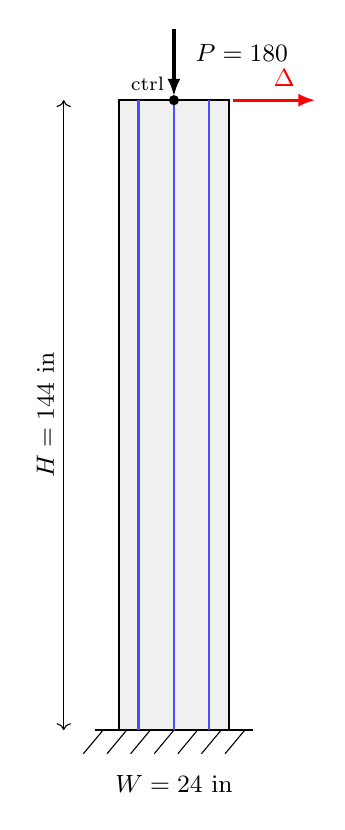
\begin{tikzpicture}[scale=1]
  \def\w{1.4}\def\h{8.0}
  \fill[gray!12] (-\w/2,0) rectangle (\w/2,\h);
  \draw[thick] (-\w/2,0) rectangle (\w/2,\h);
  \draw[thick] (-\w/2-0.3,0) -- (\w/2+0.3,0);
  \foreach \x in {-0.9,-0.6,...,0.9} { \draw (\x,0) -- (\x-0.25,-0.3); }
  \foreach \x in {-0.45,0,0.45} { \draw[blue!70,thick] (\x,0) -- (\x,\h); }
  \draw[-{Latex[length=2.2mm]},very thick] (0,\h+0.9) -- (0,\h+0.05);
  \node[right] at (0.15,\h+0.6) {\small $P=180$};
  \draw[-{Latex[length=2.2mm]},very thick,red] (\w/2+0.05,\h) -- (\w/2+1.1,\h);
  \node[red,above] at (\w/2+0.7,\h+0.05) {\small $\Delta$};
  \filldraw (0,\h) circle (1.6pt) node[above left]{\scriptsize ctrl};
  \draw[<->] (-\w/2-0.7,0) -- (-\w/2-0.7,\h);
  \node[rotate=90,above] at (-\w/2-0.7,\h/2) {\small $H=144$ in};
  \node[below] at (0,-0.45) {\small $W=24$ in};
\end{tikzpicture}
\caption{Elevation (schematic).}
\end{subfigure}\hfill
\begin{subfigure}{0.56\textwidth}
\centering
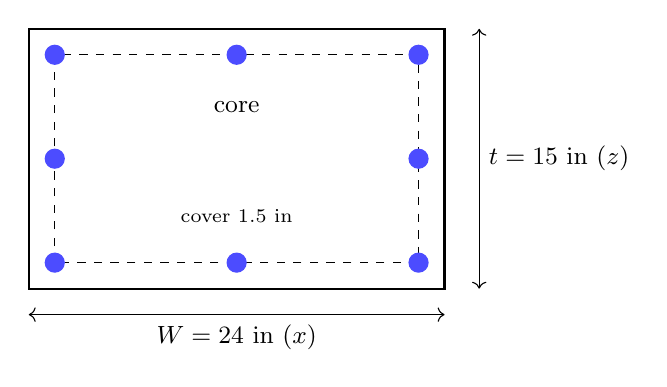
\begin{tikzpicture}[scale=0.22]
  \draw[thick] (-12,-7.5) rectangle (12,7.5);
  \draw[dashed] (-10.5,-6) rectangle (10.5,6);
  \foreach \z in {-6,0,6} { \filldraw[blue!70] (-10.5,\z) circle (0.55); }
  \foreach \z in {-6,6}    { \filldraw[blue!70] (0,\z)    circle (0.55); }
  \foreach \z in {-6,0,6} { \filldraw[blue!70] (10.5,\z)  circle (0.55); }
  \draw[<->] (-12,-9) -- (12,-9); \node[below] at (0,-9) {\small $W=24$ in ($x$)};
  \draw[<->] (14,-7.5) -- (14,7.5); \node[right] at (14,0) {\small $t=15$ in ($z$)};
  \node at (0,3) {\small core};
  \node[align=center] at (0,-3.3) {\scriptsize cover $1.5$ in};
\end{tikzpicture}
\caption{Cross-section: $A_s = 1.8 / 1.2 / 1.8\unit{in^2}$ at $x=-10.5/0/+10.5$ in.}
\end{subfigure}
\caption{Physical specimen. Lateral load and displacement $\Delta$ act along $x$ (bending about
the $z$ axis). Drawings are schematic; dimensions are labelled with their true values.}
\end{figure}

\subsection{Materials}

Concrete is defined by two physical grades --- a \emph{confined core} and an \emph{unconfined
cover} --- and the reinforcement by a single steel grade. Values are stored as positive
magnitudes; the OpenSees sign convention (compression negative) is applied in the material
mapping (Section~\ref{sec:matmap}).

\begin{table}[H]
\centering
\caption{Concrete grades (physical input). $\rho$ is mass density.}
\begin{tabular}{l c c c c c c c c}
\toprule
Grade & $E$ (ksi) & $\nu$ & $\rho$ (kip\,s$^2$/in$^4$) & $f'_c$ (ksi) & $\varepsilon_{c0}$ & $f_{cu}$ (ksi) & $\varepsilon_{U}$ & $f_t$ (ksi) \\
\midrule
Confined core    & 4030 & 0.20 & $2.25\times10^{-7}$ & 6.0 & 0.004 & 4.0 & 0.030 & 0.6 \\
Unconfined cover & 4030 & 0.20 & $2.25\times10^{-7}$ & 5.0 & 0.002 & 0.0 & 0.006 & 0.5 \\
\bottomrule
\end{tabular}
\end{table}

The Concrete02 softening shape factor is $\lambda = 0.1$ for both grades.

\begin{table}[H]
\centering
\caption{Reinforcing-steel grade (Steel02 / Giuffr\'e--Menegotto--Pinto).}
\begin{tabular}{l c c c c c c}
\toprule
Grade & $f_y$ (ksi) & $E_0$ (ksi) & $b$ & $R_0$ & $c_{R1}$ & $c_{R2}$ \\
\midrule
Reinforcement & 60.0 & 30000 & 0.01 & 18.0 & 0.925 & 0.15 \\
\bottomrule
\end{tabular}
\end{table}

\subsection{Reinforcement layout}

\begin{table}[H]
\centering
\caption{Reinforcement. Longitudinal bars lump the benchmark $3{+}2{+}3$ bars at
$0.6\unit{in^2}$ each into one area per layer; transverse ties are placed one per mesh row.}
\begin{tabular}{l l l l}
\toprule
Type & Position & Area (in$^2$) & Extent \\
\midrule
Longitudinal layer 1 & $x=-10.5$ in & 1.8 & full height $0\le y\le 144$ \\
Longitudinal layer 2 & $x=0$ in     & 1.2 & full height $0\le y\le 144$ \\
Longitudinal layer 3 & $x=+10.5$ in & 1.8 & full height $0\le y\le 144$ \\
Transverse ties      & each mesh row $y_i$ & 0.3 per tie & $x=-10.5 \to +10.5$ \\
\bottomrule
\end{tabular}
\end{table}

Total longitudinal steel area is $4.8\unit{in^2}$, identical in every model. Transverse ties
(stirrups) are present in the lattice only; the fiber and continuum references carry the
longitudinal bars only.

% ============================================================================
\section{Numerical models}
% ============================================================================

\subsection{RC lattice model (primary)}
\label{sec:lattice}

The lattice is a 2D assembly of axial struts (two translational DOFs per node) built on a
structured \code{gmsh} grid; struts connect node pairs within a peridynamic-style horizon, and
reinforcement is added as steel struts on the shared lattice nodes (perfectly bonded).

\begin{table}[H]
\centering
\caption{RC lattice model definition.}
\begin{tabular}{>{\raggedright\arraybackslash}p{4.4cm} >{\raggedright\arraybackslash}p{10.8cm}}
\toprule
Item & Specification \\
\midrule
Model dimension      & \code{ndm}=2, \code{ndf}=2 \\
Mesh generator       & \code{gmsh} structured transfinite grid \\
Mesh size            & $1.5\unit{in}$ ($16\times96$ cells) \\
Nodes                & 1649 ($17\times97$ grid) \\
Strut element        & \code{corotTruss} (corotational, geometric nonlinearity) \\
Strut connectivity   & horizon rule, $r = \text{horizon}\times\text{mesh} = 1.5\times1.5 = 2.25\unit{in}$ \\
\quad orthogonal struts & length $1.5$ in (vertical + horizontal) \\
\quad diagonal struts   & length $1.5\sqrt{2}=2.1213$ in \\
Concrete material    & per-zone length-regularized \code{Concrete02} (4 distinct) \\
Rebar material       & \code{Steel02} (1 grade) \\
Base support         & 17 base-row nodes fixed ($u_x,u_y$) \\
Control node         & top-centre node \\
\bottomrule
\end{tabular}
\end{table}

\begin{table}[H]
\centering
\caption{Lattice element inventory (7902 struts; 5 uniaxial materials).}
\begin{tabular}{l r l r}
\toprule
Concrete struts & count & Reinforcement struts & count \\
\midrule
vertical (orthogonal)   & 1632 & longitudinal (3 layers)       & 288 \\
horizontal (orthogonal) & 1552 & transverse ties (rows)        & 1358 \\
diagonal                & 3072 & & \\
\midrule
\textbf{concrete total} & \textbf{6256} & \textbf{rebar total} & \textbf{1646} \\
\bottomrule
\end{tabular}
\end{table}

\paragraph{Length-regularized concrete (crack-band).}
Both softening branches of the strut concrete law are regularized by the strut length $L$, so
that the dissipated energy is mesh-objective:
\[
E_{ts}=\frac{f_t^2 L}{2G_f}\ \ (\le 0.5E),
\qquad
\varepsilon_{U}=\varepsilon_{c0}+\frac{2G_{fc}}{(f_c+f_{cu})\,L}\ \ (\ge \varepsilon_U^{\text{grade}}),
\]
with a residual compression plateau $f_{cu}\ge 0.2 f_c$. The fracture energies are
$G_f = 4.0\times10^{-3}\unit{kip/in}$ (tension) and $G_{fc}=1.5\unit{kip/in}$ (compression).
This yields four concrete materials (two zones $\times$ two strut lengths):

\begin{table}[H]
\centering
\caption{Lattice \code{Concrete02} arguments
$(f_{pc},\varepsilon_{c0},f_{pcu},\varepsilon_{U},\lambda,f_t,E_{ts})$, compression negative.}
\begin{tabular}{l l}
\toprule
Zone / strut length & Arguments \\
\midrule
Cover, $L=1.5$    & $(-5.0,\,-0.002,\,-1.0,\,-0.33533,\,0.1,\,0.5,\,46.875)$ \\
Cover, $L=2.1213$ & $(-5.0,\,-0.002,\,-1.0,\,-0.23770,\,0.1,\,0.5,\,66.291)$ \\
Core,  $L=1.5$    & $(-6.0,\,-0.004,\,-4.0,\,-0.20400,\,0.1,\,0.6,\,67.500)$ \\
Core,  $L=2.1213$ & $(-6.0,\,-0.004,\,-4.0,\,-0.14542,\,0.1,\,0.6,\,95.459)$ \\
Rebar (Steel02)   & $(60.0,\,30000,\,0.01,\,18.0,\,0.925,\,0.15)$ \\
\bottomrule
\end{tabular}
\end{table}

\paragraph{Linear-material variant.}
For the elastic cases the concrete struts use \code{Elastic} at $E=4030\unit{ksi}$ and the rebar
struts use \code{Elastic} at $E_0=30000\unit{ksi}$; the topology and node grid are unchanged.

\paragraph{Mass.}
Nodal mass is lumped by tributary volume ($\rho\,t\,A_\mathrm{trib}/4$ per quad corner). The
total lattice self-mass is $\sum m = 1.1664\times10^{-2}\unit{kip\,s^2/in}$
($=\rho V$, $V=24\times144\times15$). For the dynamic cases a top lumped mass
$P/g = 0.4658\unit{kip\,s^2/in}$ (the axial load as tributary seismic mass) is added at the top
nodes (top/self ratio $\approx 40$).

\begin{figure}[H]
\centering
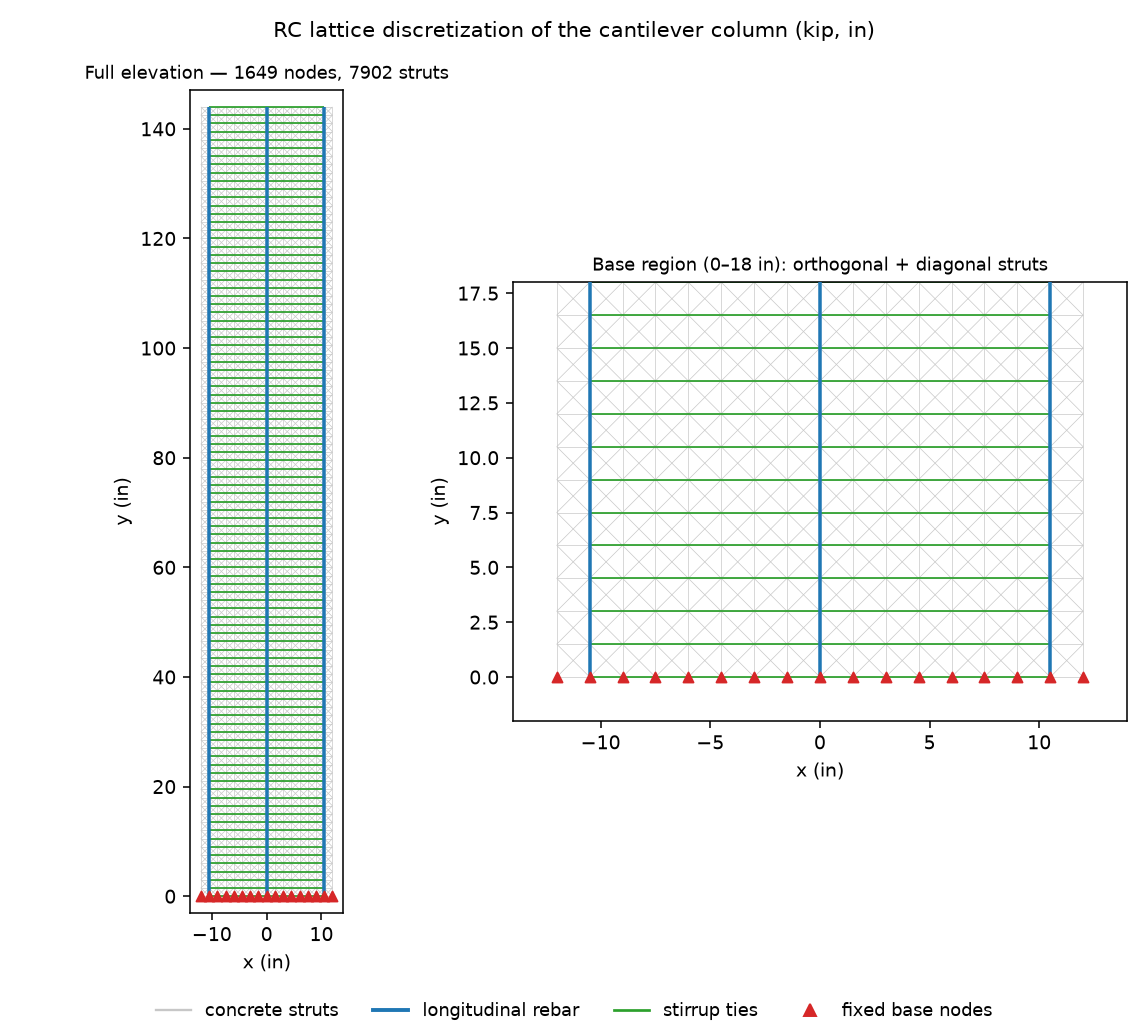
\includegraphics[width=0.86\textwidth]{column_lattice_mesh.png}
\caption{RC lattice discretization: concrete horizon struts (grey), longitudinal rebar struts
(blue), transverse stirrup ties (green), and fixed base nodes (red). Left: full elevation; right:
base region detail showing the orthogonal and diagonal strut pattern.}
\end{figure}

\subsection{Force-based fiber beam--column reference (subdivided)}
\label{sec:fiber}

The dynamic reference is a force-based \code{forceBeamColumn} fiber column in a 2D model with
three DOFs per node ($u_x,u_y,\theta_z$), subdivided into 96 equal elements (nodes at the lattice
row heights) so the self-mass distributes by tributary length identically to the lattice.

\begin{table}[H]
\centering
\caption{Fiber beam--column model definition.}
\begin{tabular}{>{\raggedright\arraybackslash}p{4.4cm} >{\raggedright\arraybackslash}p{10.8cm}}
\toprule
Item & Specification \\
\midrule
Model dimension          & \code{ndm}=2, \code{ndf}=3 \\
Element                   & \code{forceBeamColumn} \\
Number of elements       & 96 (dynamic); 1 (static pushover / single-element study) \\
Geometric transform      & \code{PDelta} \\
Beam integration         & \code{Lobatto}, 5 integration points per element \\
Fiber section            & $24$ ($y$) $\times\,15$ ($z$), cover $1.5$ in \\
\quad core patch         & $10\times1$ fibers (material: core) \\
\quad cover patches      & 1-fiber strips (material: cover) \\
\quad steel layers       & $3 / 2 / 3$ bars at $y=-10.5 / 0 / +10.5$, $A_s=0.6\unit{in^2}$ \\
Axial load               & $P=180\unit{kip}$ at the top node (held constant) \\
Self-mass (dynamic)      & distributed by tributary length; top mass $P/g$ at free top \\
\bottomrule
\end{tabular}
\end{table}

The fiber materials are matched to the lattice grades: nonlinear cases use \code{Concrete02}
(core/cover) and \code{Steel02}; linear cases use \code{Elastic} ($E=4030\unit{ksi}$ concrete,
$E_0=30000\unit{ksi}$ steel). The fiber-section \code{Concrete02} laws use the grade values
directly (no length regularization; there is no fiber analog):

\begin{table}[H]
\centering
\caption{Fiber-section \code{Concrete02} arguments
$(f_{pc},\varepsilon_{c0},f_{pcu},\varepsilon_{U},\lambda,f_t,E_{ts})$, compression negative.}
\begin{tabular}{l l}
\toprule
Fiber material & Arguments \\
\midrule
Core  (nonlinear) & $(-6.0,\,-0.004,\,-4.0,\,-0.030,\,0.1,\,0.6,\,403.0)$ \\
Cover (nonlinear) & $(-5.0,\,-0.002,\,-0.0,\,-0.006,\,0.1,\,0.5,\,403.0)$ \\
Steel (Steel02)   & $(60.0,\,30000,\,0.01,\,18.0,\,0.925,\,0.15)$ \\
\bottomrule
\end{tabular}
\end{table}

\subsection{Single-element fiber beam--column}
\label{sec:single}

The single-element model (script \code{single\_beamcolumn.py}) idealizes the fiber column as one
\code{forceBeamColumn} element with 5 Gauss--Lobatto integration points (fixed base node, free
top node), with the same fiber section and materials as Section~\ref{sec:fiber}. It serves both as
the pushover reference and the dynamic reference for that script. Because it has no interior nodes,
the column self-mass is carried as distributed element mass
(\code{massDens} $=m_\mathrm{self}/H$) and the axial-load tributary seismic mass $P/g$ is lumped
at the free top node. It is the same model OpenSees builds for the static pushover reference of
\code{pushover.py}.

\begin{figure}[H]
\centering
\includegraphics[width=0.92\textwidth]{single_beamcolumn/single_beamcolumn_pushover_bc_model.png}
\caption{Single-element fiber beam--column: column elevation (5 Lobatto points, fixed base,
top node) and the fiber section (core/cover patches and longitudinal rebar).}
\end{figure}

\subsection{2D plane-stress continuum reference}
\label{sec:continuum}

The continuum reference is a structured plane-stress quad mesh of the same column, with nonlinear
nD concrete and the longitudinal bars represented as steel struts sharing the quad nodes.

\begin{table}[H]
\centering
\caption{2D continuum model definition.}
\begin{tabular}{>{\raggedright\arraybackslash}p{4.4cm} >{\raggedright\arraybackslash}p{10.8cm}}
\toprule
Item & Specification \\
\midrule
Model dimension      & \code{ndm}=2, \code{ndf}=2 (plane stress, thickness $t=15$ in) \\
Mesh generator       & \code{gmsh} structured grid, mesh size $1.5\unit{in}$ \\
Nodes                & 1649 \\
Elements             & 1824 total: 1536 plane-stress quads + 288 longitudinal rebar struts \\
Concrete material    & \code{ASDConcrete3D} + \code{PlaneStress} wrapper, per zone (4 nD materials) \\
Rebar material       & \code{Steel02} (1 uniaxial), longitudinal bars only (no stirrups) \\
Regularization       & crack-band by element characteristic length $l_{ch}=1.5\unit{in}$ \\
Hysteresis setting   & pure damage (\code{plastic\_frac}$=0$, $d_{\max}=0.95$) \\
Base support         & 17 base-row nodes fixed ($u_x,u_y$) \\
Control node         & top-centre node (id 873) \\
\bottomrule
\end{tabular}
\end{table}

\code{ASDConcrete3D} is driven by uniaxial tension ($Te/Ts/Td$) and compression ($Ce/Cs/Cd$)
curves given as positive magnitudes; damage values $d$ follow from
$d=\mathrm{clip}(1-\sigma/(E\varepsilon),0,d_{\max})$ (pure damage, $\code{plastic\_frac}=0$):

\begin{table}[H]
\centering
\caption{Continuum \code{ASDConcrete3D} curves ($E=4030\unit{ksi}$, $\nu=0.2$, $l_{ch}=1.5$ in).
Strain / stress (ksi) / damage triples.}
\small
\begin{tabular}{l l l}
\toprule
Branch & Core & Cover \\
\midrule
$Te$ (strain) & $0,\ 1.49\!\times\!10^{-4},\ 9.038\!\times\!10^{-3}$ & $0,\ 1.24\!\times\!10^{-4},\ 1.0791\!\times\!10^{-2}$ \\
$Ts$ (ksi)    & $0,\ 0.6,\ 0.012$ & $0,\ 0.5,\ 0.010$ \\
$Td$          & $0,\ 0,\ 0.95$ & $0,\ 0,\ 0.95$ \\
$Ce$ (strain) & $0,\ 5.96\!\times\!10^{-4},\ 4.0\!\times\!10^{-3},\ 0.204$ & $0,\ 4.96\!\times\!10^{-4},\ 2.0\!\times\!10^{-3},\ 0.402$ \\
$Cs$ (ksi)    & $0,\ 2.4,\ 6.0,\ 4.0$ & $0,\ 2.0,\ 5.0,\ 0.0$ \\
$Cd$          & $0,\ 0,\ 0.6278,\ 0.95$ & $0,\ 0,\ 0.3797,\ 0.95$ \\
\bottomrule
\end{tabular}
\end{table}

% ============================================================================
\section{Material mapping summary}
\label{sec:matmap}
% ============================================================================

\begin{table}[H]
\centering
\caption{Physical grade $\to$ per-model OpenSees material.}
\begin{tabular}{l l l}
\toprule
Use & Nonlinear & Linear (elastic) \\
\midrule
Lattice concrete strut       & length-regularized \code{Concrete02} & \code{Elastic} ($E$) \\
Lattice / fiber / quad rebar & \code{Steel02} & \code{Elastic} ($E_0$) \\
Fiber-section concrete       & plain \code{Concrete02} (grade values) & \code{Elastic} ($E$) \\
Continuum concrete           & \code{ASDConcrete3D} + \code{PlaneStress} & --- \\
\bottomrule
\end{tabular}
\end{table}

% ============================================================================
\section{Stiffness calibration}
\label{sec:calib}
% ============================================================================

The single calibration parameter is the concrete strut cross-sectional area $A$ (uniform over all
concrete struts), chosen so the lattice's initial lateral stiffness $K_0$ equals the chosen
reference's. The reinforcement areas are fixed by the specimen and are not calibrated.

\begin{itemize}
\item \textbf{Nonlinear cases:} a plain elastic lattice (reinforcement omitted) has
      $K_0 \propto A$, so a single solve gives $A$ from the reference $K_0$.
\item \textbf{Linear cases:} the full RC elastic lattice (concrete $+$ rebar) has a stiffness that
      is monotone but not proportional in $A$ (rebar adds a parallel stiffness), so $A$ is found by
      a secant root-find on $K_0(A)-K_0^{\mathrm{ref}}$.
\end{itemize}

\begin{table}[H]
\centering
\caption{Calibration results. $K_0^{\mathrm{ref}}$ is the reference's initial lateral stiffness
(first finite pushover step).}
\begin{tabular}{l l c c}
\toprule
Configuration & Reference & $K_0^{\mathrm{ref}}$ (kip/in) & Calibrated $A$ (in$^2$) \\
\midrule
Linear            & fiber beam--column            & 68.69 & 11.736 \\
Nonlinear         & fiber BC (single \& subdivided) & 61.53 & 12.453 \\
Nonlinear         & 2D continuum                  & 80.34 & 16.260 \\
\bottomrule
\end{tabular}
\end{table}

For the linear calibration the resulting lattice $K_0 = 68.69\unit{kip/in}$ ($-0.00\%$ vs.\ the
reference). The continuum reference yields a larger $A$ (and a stiffer, shorter-period lattice)
than the fiber reference because $K_0^{\mathrm{ref}}$ is larger.

% ============================================================================
\section{Analysis types and parameters}
% ============================================================================

\subsection{Pushover}
\label{sec:proc-pushover}

A constant-gravity stage (axial $P$) is applied first and held; the lateral displacement of the
control node is then increased monotonically under displacement control while the base shear
(sum of horizontal base reactions) is recorded.

\begin{table}[H]
\centering
\caption{Pushover analysis parameters (all models).}
\begin{tabular}{>{\raggedright\arraybackslash}p{4.4cm} >{\raggedright\arraybackslash}p{10.8cm}}
\toprule
Item & Setting \\
\midrule
Constraint handler   & \code{Transformation} \\
DOF numberer         & \code{RCM} \\
System of equations  & \code{BandGeneral} \\
Gravity stage        & \code{LoadControl}, 10 steps; \code{Newton}; \code{NormDispIncr} $10^{-8}$ \\
Hold gravity         & \code{loadConst} (time reset to 0) \\
Lateral stage        & \code{DisplacementControl} on control DOF, $dU=0.05\unit{in}$ \\
Target tip displacement & $10.0\unit{in}$ \\
Convergence test     & \code{NormDispIncr}, tol $10^{-5}$ (lattice), $10^{-6}$ (fiber) \\
Primary algorithm    & \code{Newton} \\
Recovery on failure  & sub-steps $5/20/100$ with
                       \code{Newton}$\to$\code{KrylovNewton} \\
Base shear           & $-\sum$ horizontal base reactions \\
\bottomrule
\end{tabular}
\end{table}

\subsection{Dynamic (seismic time history)}
\label{sec:proc-dynamic}

After the held-gravity stage, the base is driven by a \code{UniformExcitation} (ground
acceleration record) along $x$. The record intensity is tuned on the (inexpensive) fiber column to
a target peak roof drift; the \emph{same} scaled record then drives the lattice (and, for the
continuum cases, the continuum). Two records are used per case: a harmonic acceleration tuned to
resonance with the lattice fundamental period $T_1$, and the recorded El Centro 1940 NS ground
motion.

\begin{table}[H]
\centering
\caption{Dynamic analysis parameters (all models).}
\begin{tabular}{>{\raggedright\arraybackslash}p{4.4cm} >{\raggedright\arraybackslash}p{10.8cm}}
\toprule
Item & Setting \\
\midrule
Constraint handler / numberer / system & \code{Transformation} / \code{RCM} / \code{BandGeneral} \\
Mass                 & lumped self-mass $+$ top mass $P/g$ \\
Damping              & \textbf{modal damping}, $5\%$ at modes 1 and 2 \\
Time integrator      & \code{HHT}, $\alpha=0.7$ (numerical damping) \\
Integration step     & $\Delta t = 0.005\unit{s}$ (nonlinear); $0.01\unit{s}$ (linear) \\
Convergence test     & \code{NormDispIncr}, tol $10^{-6}$, 50 iterations \\
Primary algorithm    & \code{Newton} \\
Recovery on failure  & sub-steps $10/50/200$ with \code{Newton}$\to$\code{KrylovNewton}
                       $\to$\code{NewtonLineSearch}(Bisection)$\to$\code{ModifiedNewton} \\
Excitation pattern   & \code{UniformExcitation} along $x$ \\
Target peak drift (tuning) & $1.0\unit{in}$ (linear); $2.0\unit{in}$ (nonlinear) \\
\bottomrule
\end{tabular}
\end{table}

\begin{table}[H]
\centering
\caption{Base excitation records. The sine period equals the lattice $T_1$ (resonant); the
continuum sine case is capped at 8 cycles.}
\begin{tabular}{l l l l l}
\toprule
Record & Points & $\Delta t_\mathrm{rec}$ (s) & Peak (g) & Duration (s) \\
\midrule
Sine resonance (20 cycles, 100 samples/cycle) & 2001 & $T_1/100$ & 1.000 & $20\,T_1$ \\
Sine resonance (8 cycles, continuum)          & 801  & $T_1/100$ & 1.000 & $8\,T_1$ \\
El Centro 1940 NS & 1559 & 0.0200 & 0.319 & 31.2 \\
\bottomrule
\end{tabular}
\end{table}

The continuum dynamic reference uses \code{ASDConcrete3D} configured as pure damage
($\code{plastic\_frac}=0$); it is computationally heavy ($\approx 1.5$ s/step over 1536 quads),
hence the 8-cycle sine cap.

% ============================================================================
\section{Results}
% ============================================================================

\subsection{Pushover}
\label{sec:res-pushover}

\begin{figure}[H]
\centering
\begin{subfigure}{0.32\textwidth}
\centering
\includegraphics[width=\textwidth]{pushover_linear/beamcolumn/column_pushover_linear.png}
\caption{Linear (elastic), fiber reference.}
\end{subfigure}\hfill
\begin{subfigure}{0.32\textwidth}
\centering
\includegraphics[width=\textwidth]{pushover/beamcolumn/column_pushover_beamcolumn.png}
\caption{Nonlinear, fiber reference.}
\end{subfigure}\hfill
\begin{subfigure}{0.32\textwidth}
\centering
\includegraphics[width=\textwidth]{pushover/continuum/column_pushover_continuum.png}
\caption{Nonlinear, continuum reference.}
\end{subfigure}
\caption{Base shear versus tip displacement: RC lattice (blue, dashed) and the reference (red).}
\end{figure}

\begin{table}[H]
\centering
\caption{Pushover results. Peak shear is the maximum recorded base shear; max tip displacement is
the last converged step.}
\small
\setlength{\tabcolsep}{5pt}
\begin{tabular}{l l c c c}
\toprule
Configuration & Model & Peak shear (kip) & Max tip disp.\ (in) & Converged \\
\midrule
\multirow{2}{*}{Linear (fiber ref.)}
 & Fiber beam--column & 686.9 (@10 in) & 10.00 & yes \\
 & RC lattice         & 690.2 (@10 in) & 10.00 & yes \\
\midrule
\multirow{2}{*}{Nonlinear (fiber ref.)}
 & Fiber beam--column & 31.37 & 10.00 & yes \\
 & RC lattice         & 36.75 & 6.17  & no (terminated) \\
\midrule
\multirow{2}{*}{Nonlinear (continuum ref.)}
 & 2D continuum       & 39.12 & 9.28 & no (terminated) \\
 & RC lattice         & 39.80 & 5.50 & no (terminated) \\
\bottomrule
\end{tabular}
\end{table}

\subsection{Dynamic --- linear (elastic), fiber reference}

\noindent\textbf{Sine resonance} (scale $0.039\times$, $\Delta t=0.01$ s).
\begin{figure}[H]\centering
\includegraphics[width=\textwidth]{dynamic_linear/beamcolumn/column_dynamic_linear_sine.png}
\caption{Linear, sine --- response histories (roof drift, base shear): RC lattice vs.\ elastic
fiber beam--column.}
\end{figure}
\begin{figure}[H]\centering
\includegraphics[width=\textwidth]{dynamic_linear/beamcolumn/column_dynamic_linear_sine_hyst.png}
\caption{Linear, sine --- hysteresis: RC lattice (left), fiber beam--column (middle), overlaid (right).}
\end{figure}

\noindent\textbf{El Centro 1940 NS} (scale $0.413\times$, $\Delta t=0.01$ s).
\begin{figure}[H]\centering
\includegraphics[width=\textwidth]{dynamic_linear/beamcolumn/column_dynamic_linear_elcentro.png}
\caption{Linear, El Centro --- response histories (roof drift, base shear).}
\end{figure}
\begin{figure}[H]\centering
\includegraphics[width=\textwidth]{dynamic_linear/beamcolumn/column_dynamic_linear_elcentro_hyst.png}
\caption{Linear, El Centro --- hysteresis: RC lattice (left), fiber beam--column (middle), overlaid (right).}
\end{figure}

\subsection{Dynamic --- nonlinear, fiber beam--column reference}

\noindent\textbf{Sine resonance} (scale $0.154\times$, $\Delta t=0.005$ s).
\begin{figure}[H]\centering
\includegraphics[width=\textwidth]{dynamic/beamcolumn/column_dynamic_beamcolumn_sine.png}
\caption{Nonlinear, sine --- response histories: RC lattice vs.\ fiber beam--column.}
\end{figure}
\begin{figure}[H]\centering
\includegraphics[width=\textwidth]{dynamic/beamcolumn/column_dynamic_beamcolumn_sine_hyst.png}
\caption{Nonlinear, sine --- hysteresis: RC lattice (left), fiber beam--column (middle), overlaid
(right). Note the separate vertical scales.}
\end{figure}

\noindent\textbf{El Centro 1940 NS} (scale $0.545\times$, $\Delta t=0.005$ s).
\begin{figure}[H]\centering
\includegraphics[width=\textwidth]{dynamic/beamcolumn/column_dynamic_beamcolumn_elcentro.png}
\caption{Nonlinear, El Centro --- response histories.}
\end{figure}
\begin{figure}[H]\centering
\includegraphics[width=\textwidth]{dynamic/beamcolumn/column_dynamic_beamcolumn_elcentro_hyst.png}
\caption{Nonlinear, El Centro --- hysteresis: RC lattice (left), fiber beam--column (middle),
overlaid (right). Note the separate vertical scales.}
\end{figure}

\subsection{Dynamic --- nonlinear, 2D continuum reference}

\noindent\textbf{Sine resonance} (scale $0.312\times$, 8 cycles, $\Delta t=0.005$ s).
\begin{figure}[H]\centering
\includegraphics[width=\textwidth]{dynamic/continuum/column_dynamic_continuum_sine.png}
\caption{Nonlinear, sine --- response histories: RC lattice vs.\ 2D continuum.}
\end{figure}
\begin{figure}[H]\centering
\includegraphics[width=\textwidth]{dynamic/continuum/column_dynamic_continuum_sine_hyst.png}
\caption{Nonlinear, sine --- hysteresis: RC lattice (left), 2D continuum (middle), overlaid (right).}
\end{figure}

\noindent\textbf{El Centro 1940 NS} (scale $0.545\times$, $\Delta t=0.005$ s).
\begin{figure}[H]\centering
\includegraphics[width=\textwidth]{dynamic/continuum/column_dynamic_continuum_elcentro.png}
\caption{Nonlinear, El Centro --- response histories.}
\end{figure}
\begin{figure}[H]\centering
\includegraphics[width=\textwidth]{dynamic/continuum/column_dynamic_continuum_elcentro_hyst.png}
\caption{Nonlinear, El Centro --- hysteresis: RC lattice (left), 2D continuum (middle), overlaid (right).}
\end{figure}

\subsection{Single-element beam--column study}

Script \code{single\_beamcolumn.py} compares the RC lattice against the single-element fiber
beam--column (Section~\ref{sec:single}) under both a nonlinear pushover (same machinery as
Section~\ref{sec:proc-pushover}) and a nonlinear seismic time-history (Section~\ref{sec:proc-dynamic},
$\Delta t=0.005$ s).

\noindent\textbf{Pushover.}
\begin{figure}[H]\centering
\includegraphics[width=0.55\textwidth]{single_beamcolumn/single_beamcolumn_pushover.png}
\caption{Pushover --- base shear versus tip displacement: RC lattice vs.\ single-element fiber
beam--column.}
\end{figure}

\noindent\textbf{Sine resonance} (scale $0.312\times$).
\begin{figure}[H]\centering
\includegraphics[width=\textwidth]{single_beamcolumn/single_beamcolumn_sine.png}
\caption{Single-element, sine --- response histories.}
\end{figure}
\begin{figure}[H]\centering
\includegraphics[width=\textwidth]{single_beamcolumn/single_beamcolumn_sine_hyst.png}
\caption{Single-element, sine --- hysteresis: RC lattice (left), single beam--column (middle),
overlaid (right).}
\end{figure}

\noindent\textbf{El Centro 1940 NS} (scale $0.750\times$).
\begin{figure}[H]\centering
\includegraphics[width=\textwidth]{single_beamcolumn/single_beamcolumn_elcentro.png}
\caption{Single-element, El Centro --- response histories.}
\end{figure}
\begin{figure}[H]\centering
\includegraphics[width=\textwidth]{single_beamcolumn/single_beamcolumn_elcentro_hyst.png}
\caption{Single-element, El Centro --- hysteresis: RC lattice (left), single beam--column (middle),
overlaid (right).}
\end{figure}

\subsection{Tabulated dynamic results}

\begin{table}[H]
\centering
\caption{Dynamic results. $T_1$ is the lattice fundamental period (and the sine excitation period);
drift is the relative roof displacement; peak $|V|$ is the maximum absolute recorded base shear
(includes transient reaction peaks); residual is the end-of-record roof drift.}
\small
\setlength{\tabcolsep}{4pt}
\begin{tabular}{l l c c c c c c c}
\toprule
\multirow{2}{*}{Study / record} & \multirow{2}{*}{Scale} & \multirow{2}{*}{$T_1$ (s)}
 & \multicolumn{2}{c}{Peak drift (in)} & \multicolumn{2}{c}{Peak $|V|$ (kip)} & \multicolumn{2}{c}{Residual (in)} \\
\cmidrule(lr){4-5}\cmidrule(lr){6-7}\cmidrule(lr){8-9}
 & & & Ref. & Lattice & Ref. & Lattice & Ref. & Lattice \\
\midrule
Linear, sine            & $0.039\times$ & 0.515 & 1.000 & 0.990 & 68.7 & 67.8 & $+0.968$ & $+0.953$ \\
Linear, El Centro       & $0.413\times$ & 0.515 & 1.000 & 0.995 & 68.5 & 68.0 & $-0.021$ & $-0.020$ \\
\midrule
Nonlinear (fiber), sine      & $0.154\times$ & 0.506 & 1.329 & 1.274 & 180.4 & 38.5 & $+0.392$ & $+0.304$ \\
Nonlinear (fiber), El Centro & $0.545\times$ & 0.506 & 1.179 & 1.391 & 206.3 & 40.1 & $+0.015$ & $+0.073$ \\
\midrule
Nonlinear (continuum), sine      & $0.312\times$ & 0.452 & 1.394 & 1.636 & 39.0 & 47.4 & $+0.386$ & $+0.462$ \\
Nonlinear (continuum), El Centro & $0.545\times$ & 0.452 & 0.857 & 1.222 & 36.0 & 41.9 & $-0.148$ & $+0.011$ \\
\midrule
Single BC, sine         & $0.312\times$ & 0.506 & 1.915 & 1.801 & 31.9 & 39.0 & $+0.132$ & $+0.516$ \\
Single BC, El Centro    & $0.750\times$ & 0.506 & 1.809 & 1.664 & 32.0 & 39.2 & $-0.096$ & $+0.027$ \\
\bottomrule
\end{tabular}
\end{table}

The fiber-proxy fundamental period used to tune the intensity is $T_1^{\mathrm{fiber}}=0.520$ s
(linear), $0.558$ s (nonlinear subdivided), and $0.559$ s (single element).

% ============================================================================
\appendix
\section{Software and reproduction}
% ============================================================================

\begin{table}[H]
\centering
\caption{Software environment (native arm64, macOS).}
\begin{tabular}{l l}
\toprule
Component & Version \\
\midrule
Python        & 3.12.13 (arm64) \\
openseespy    & 3.8.0.0 (openseespymac 3.8.0.0) \\
gmsh          & 4.15.2 \\
numpy / scipy & 2.4.6 / 1.17.1 \\
matplotlib    & 3.11.0 \\
\bottomrule
\end{tabular}
\end{table}

Run from the \code{src/} directory with the project virtual environment active:

{\small
\begin{verbatim}
python examples/column/pushover_linear.py
python examples/column/pushover.py        --reference beamcolumn
python examples/column/pushover.py        --reference continuum
python examples/column/dynamic_linear.py  --excitation sine
python examples/column/dynamic_linear.py  --excitation elcentro
python examples/column/dynamic.py         --reference beamcolumn --excitation sine
python examples/column/dynamic.py         --reference beamcolumn --excitation elcentro
python examples/column/dynamic.py         --reference continuum  --excitation sine
python examples/column/dynamic.py         --reference continuum  --excitation elcentro
python examples/column/single_beamcolumn.py --analysis pushover
python examples/column/single_beamcolumn.py --analysis dynamic --excitation sine
python examples/column/single_beamcolumn.py --analysis dynamic --excitation elcentro
python examples/doc/make_model_figures.py   # lattice mesh figure
\end{verbatim}
}

Drawings of every analysis model are written next to each result (the \code{*\_model.png} files);
add \code{--draw} where the script supports it.

\end{document}
